\chapter{Background}
\label{chp:background} 

\section{Village Telco}
The Village Telco concept was developed in June 2008 during a workshop at the Shuttleworth Foundation in Cape Town, South Africa. The main goal was to develop an inexpensive system to provide rural and under-served areas with affordable telephone communication \cite{MParticle}. The workshop included participants like open hardware pioneer Dawid Rowe, and Elektra, the developer of B.A.T.M.A.N (for more information about B.A.T.M.A.N see section \ref{subsec:batman}) \cite{MPworkshop}. The purpose of the workshop was to develop a business model, as well as a prototype for a Village Telco. Initially the idea was to use low cost \gls{voip} headsets. At that time it was the most viable and convenient way to deliver telephone services to the customers. The wireless VoIP telephones have small antennas, which became a problem. The nodes could not be more than 100 meters away from each other in order to have a reliable connection. This required more nodes in order to cover a desirable area. This factor drastically increased the start-up costs for a village. In order to keep the cost down, it was also important to keep the number of access points (APs) down. A mesh network has a larger range, and one suggestion was to use a small mesh device like an Open Mesh AP and connect a SIP phone to it. This solution would solve a lot of the problems regarding range, antenna and number of access points, but the idea was still an expensive option. The challenge was to create something that would be simple enough to be configured, and scaled by local entrepreneurs with limited technical skills. In addition to this it was important to keep the cost down. The two key cost factors that emerged in the scale-up of a Village Telco were the cost of the customer's phone and the power supply. It was clear that the power supply was the most important factor, and that they had to look at other, and cheaper options regarding the customers phones \cite{MPworkshop}. During the debating, Rael Lissoos took an Analogue Telephone Adapter (ATA) and an Open Mesh AP, held them together and said; \textit{"we need these two devices in one"}. This point was the birth of the Mesh Potato, fully based on customized open hardware and software design. The name "Mesh Potato" comes from combining the words mesh, POTS (Plain Old Telephone) and ATA. "Patata" is the Spanish word for potato, and hence the name Mesh Potato. The Mesh Potato is a mesh enabled Wi-Fi device, with the possibility to connect any inexpensive regular phone and IP device \cite{MPorigin}.


\section{Mesh Potato}

\begin{figure}[b]
  \centering
      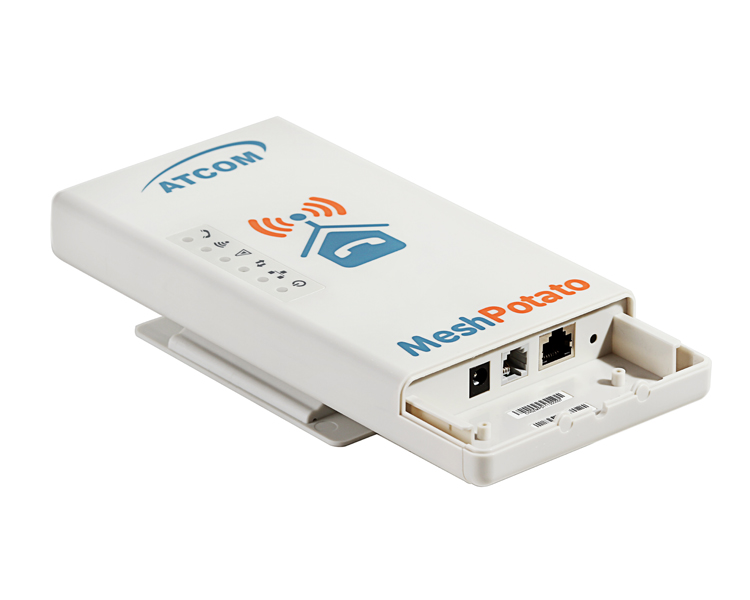
\includegraphics[width=0.5\textwidth]{MP01}
  \caption [MP01]{\textbf{The first generation Mesh Potato, MP01.}}
  \label{fig:MP01}
\end{figure}

The first generation of the Mesh Potato is shown in \fref{fig:MP01}. This device was designed to be used in rural areas. It can be deployed and run anywhere in the world, relying only on a low, but stable, power supply. The Ethernet port, the Foreign eXchange Station (FXS) ports, and the power port are robust and designed in order to handle all weather conditions, poor power conditions, lightening and static electricity. In addition to this, the Mesh Potato comes in a waterproof box for outdoor mounting \cite{background}.

The Mesh Potato combines the features of a 802.11bg Wi-Fi router with an Analogue Telephone Adaptor (ATA) \cite{MP}. The ATA converts the signal from a standard telephone, into the digital signal needed to connect to the Internet and use the SIP protocol \cite{MParticle}. The device is based on the Atheros chipset that is used by OpenMesh, and runs OpenWrt (see section \ref{subsec:openwrt} for more information) and B.A.T.M.A.N. (see section \ref{subsec:batman} for more information). Each Mesh Potato provides a single fixed telephone line to the end user. The MPs are connected together via a mesh Wi-Fi network, and configure themselves automatically to form a peer-to-peer network, greatly extending the range of the network over regular Wi-Fi. This enables the phone calls to be made independent of landlines and telephone towers, and creates the basis for the "plug-and-play" solution. 

As mentioned, the Mesh Potato is based on open hardware, as well as open software design. Everything is kept open in order for any third party to test, set standards, and give feedback. Key goals during the development was to minimize the binary blobs (a closed source binary-only driver that has no publicly available source code \cite{binaryBolb}), minimize closed software and make the hardware open. 

The mesh network can be connected via a backbone link to the rest of the world by using VoIP gateways. No cell phone towers, no land lines, and no telecommunication companies are required. A Village Telco is a community owned telephone service, allowing a local entrepreneur to roll out the Village Telco system only needing a server and the wanted amount of Mesh Potatoes. The mesh network is self-healing and self-organizing, meaning if one node goes down, B.A.T.M.A.N. routes the calls through other available nodes in the network \cite{MPbyRowe}. In order to provide Internet to the mesh network, one of the Mesh Potatoes must be provided with Internet access. The internet signal enters the server in the Village Telco, this could for example be an existing internet café, with a broadband, link or satellite connection. The signal is transmitted to the super node. The super node consists of three external access points, and is placed high over ground, giving 360 degree coverage, with approximately 1 km range. The internet signal is then carried through the network from one Mesh Potato to another. 


\subsubsection{Mesh Potato 2.0}
The first generation of the Mesh Potato has sold over 2500 copies, and is deployed all over the world. In order to keep up with time, the constant technical development and the demand from the users, a new version of the Mesh Potato was introduced. The second generation became available to users August 2013. This device comes in a smaller box, as shown in \fref{fig:MP02}, and is sold to half the price of the first generation. One of the biggest differences is that the second generation has two Ethernet ports and is built on a new, and faster, chipset. It is also  operating on new firmware.

\begin{figure}[h!]
  \centering
      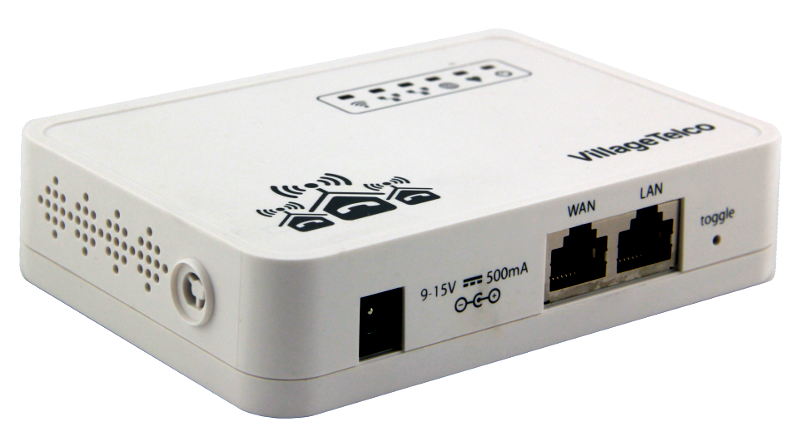
\includegraphics[width=0.5\textwidth]{mp2.PNG}
  \caption [MP2]{\textbf{The second generation Mesh Potato, MP2.}}
  \label{fig:MP02}
\end{figure}


The second generation Mesh Potatoes comes in three versions, where just the first one, MP2 Basic, is available on the market. In May/June 2014 Village Telco will release MP2 - Phone. This version will be identical to the MP2 - Basic with an FXS daughterboard, which enables the possibility to connect a phone to the MP. Village Telco will also release an advanced version of the second generation. This MP2 - AWD will be a full outdoor unit which are designed for rugged use and will have a PoE/TL adaptor which will carry voice, data and power. Time for release of this advanced version is still unannounced. 

\section{Village Telco Network Deployments} \label{sec:deployments}
There are Village Telcos in different places in the world. The first Village Telco network was established in Dili on Timor-Leste. There are also Village Telco networks in Brazil, South Africa, Nigeria, Nepal, Puerto Rico and other countries in the world. This section will present some of the villages that exist today. \fref{fig:map_deployments} show where some of the Village Telco deployments are located in the world. Since the villages are not deployed by Village Telco itself, but by local entrepreneurs, there does not exist a complete overview over all the villages. 


\begin{figure}[H]
\centering
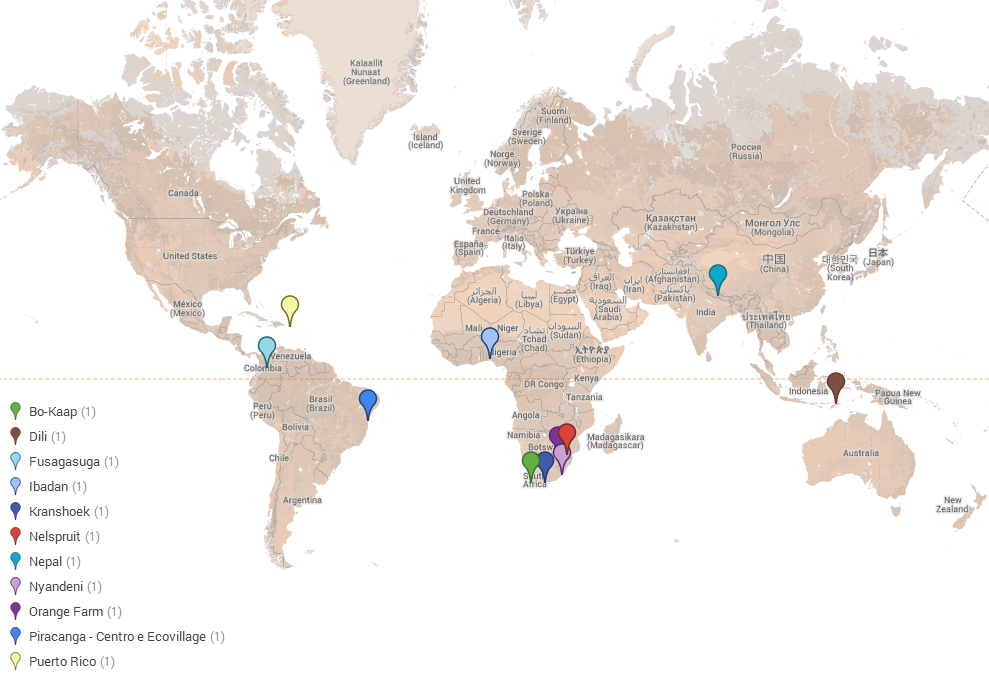
\includegraphics[width=1\textwidth]{villagetelco3.PNG}
\caption [World map of Village Telco deployments]{\textbf{World map of Village Telco deployments}}
\label{fig:map_deployments}
\end{figure}

The information about the villages that are presented in this section is gathered from the Village Telco website\cite{village_telco_deployments} and a questionnaire that was sent out on Village Telco's mailing list in February 2014 (see Section \ref{sec:survey} for more information).

\subsection{Dili, Timor-Leste}\label{sec:timor}
Dili is the capital of Timor-Leste, one of the poorest countries in Asia \cite{vt_dili}. There lives 193 000 (2010) in Dili. Over 70\% of Timor-Leste's population lives in rural areas \cite{quandl_timor}.  Timor-Leste gained its independence from Indonesia in 2002, but the telecommunications infrastructure was destroyed in the process. 


\subsubsection{Telecommunications in Timor-Leste}
There exist some infrastructure for fixed and mobile telephone in Timor-Leste. However, the services are expensive and the regular Timorese can't afford to use the services on a regular basis. After the independence of Indonesia, Timor-Leste's telecommunications sector has expanded, especially the mobile telephone sector. \fref{fig:cellular_timor} and \fref{fig:internet_timor} show number of subscriptions/users per 100 people in Timor-Leste for cellular telephony and internet. \fref{fig:internet_timor} show that there are less than 1 of 100 people that use the internet. The main reason for these low numbers are the high costs for the services in combination with low income of Timor-Leste's inhabitants. 


%\begin{figure}[H]
%\centering
%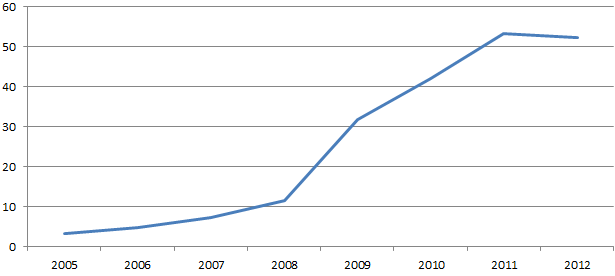
\includegraphics[width=1\textwidth]{Cellular_timor.PNG}
%\caption[Number of cellular subscriptions per 100 people in Timor-Leste]{\textbf{Number of cellular subscriptions per 100 people in Timor-Leste}}
%\label{fig:cellular_timor}
%\end{figure}

\paragraph{Telephony: }
From 2002 to 2013 Timor Telecom (owned by Portugal Telecom) had monopoly. Portugal Telecom signed a contract with the government in 2002 to invest \$29 million to rebuild and operate the phone system and giving them an exclusive license in the market until 2017 \cite{wiki_telecom_east_timor}. The contract was renewable, but in 2012 Portugal Telecom agreed with the government to end the monopoly earlier than planned\cite{budde}. In 2013 two new competitors entered the market. After this the market changed rapidly. In addition to this the government are in the process of setting up a new independent regulatory authority for the telecom sector. 

\paragraph{Internet:} There is only one \gls{isp} in Timor-Leste, Timor Telecom\cite{wiki_telecom_east_timor}. The internet traffic is expensive due to the fact that international traffic goes via expensive \gls{vsat} connections. This accounts for most of the national traffic as well \cite{vt_dili}. For example it is not possible to send a \gls{ip} packet from one side of Dili to the other without sending the packet overseas via \gls{vsat} connections. 


%\begin{figure}[H]
%\centering
%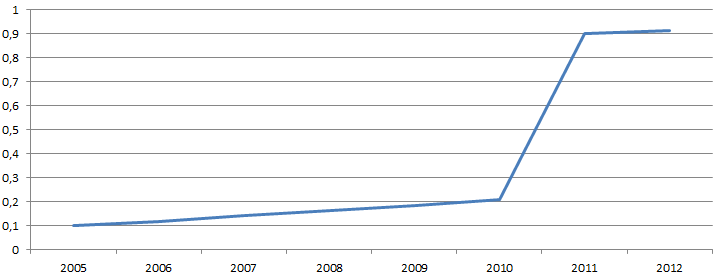
\includegraphics[width=1\textwidth]{internet_timor.PNG}
%\caption[Number of internet users per 100 people in Timor-Leste]{\textbf{Number of internet users per 100 people in Timor-Leste}}
%\label{fig:internet_timor}
%\end{figure}

\subsubsection{The Deployment}
The Village Telco deployment in Dili is planning to build a 100-node network. The project is collaboration between Rowotel \footnote{A business operated by David Rowe that focus on open telephony software and hardware} and Fongtil \footnote{The umbrella organisation for Timor-Leste’s local, national and international \glspl{ngo} }. The project was funded by \gls{isif} and \gls{isoc} community grants. 

The project had three main goals\cite{vt_dili}:
\begin{itemize}
\item Train Timorese to roll out a Village Telco network and in technologies that are necessary (mesh Wi-Fi, \gls{voip}, mesh node installation and maintenance).
\item Deploy a 100-node Village Telco network to build a local telephone network.
\item Use the mesh Wi-Fi network to provide a community \gls{ip} backbone across metropolitan Dili to encourage local \gls{ip} traffic and local content.
\end{itemize}

In May 2012 the project had 60 operating nodes, and Fongtil maintains the network. The network is a public resource, anyone in Dili has access to the bandwidth. Fongtil also trains people in \gls{mp} set up. 


\subsubsection{Business Model}
The business model in for the Village Telco deployment in Dili is based on free internal calls, in addition to pre-paid usage charging.  

\subsection{Orocovis, Puerto Rico}
Orocovis is a village in Puerto Rico with about 25 000 inhabitants. Orocovis is a rural and low-income town, the average income in the town is less than \$14 000 annually, most families require financial assistance from government funding.   

In the village there are landline telephone infrastructure that needs repair and upgrades. The village is situated in a mountainous terrain, which provides an obstacle for cellular telephony. Most of the cell phone users have to travel 30 to 40 minutes to get a stable cell phone connection \cite{vt_puerto_rico, soto}. 

\subsubsection{The Deployment}
In 2012 Jose Soto rolled out a Village Telco network in the village. Jose Soto is the president of CoquiTel, a small \gls{wisp}. CoquiTel is a project created to improve the infrastructure of Puerto Rico especially in rural or the last mile areas. The hope through the project is to create and maintain the infrastructure at the same time stimulate the local economy and provide adequate means for students in school, patients in the medical care institutions and general public as a whole.  

The network consists of 146 \glspl{mp} and are still growing as there is a plan of an expansion to other villages close to Orocovis. The deployment is mainly funded by Jose Soto\cite{vt_puerto_rico}. The initial roll out of 45 \glspl{mp} took between eight and ten months. In the beginning the main focus of the project was telephony, but this changed to Internet connectivity because the project gained access to a microwave link with a large capacity. 

\subsubsection{Business Model}
The business model of Orocovis is based on post-pay unlimited data plans and phone plans. 85\% of the service is internet and 15\% is telephony. 

\subsection{Mataffin-Macadamia, Nelspruit South Africa}
Mataffin-Macadamia is located in Nelspruit in northeast of South Africa. Mataffin-Macadamia is a retirement secure estate, and the inhabitants are of the upper middle class lifestyle. The estate consists of over 250 homes spread over a 17-hectare village. 

\subsubsection{The Deployment}
Mataffin-Macadamia offers telephony and Internet with use of Village Telco's technology\cite{mataffin_ict}. There are 45 \glspl{mp} installed so far in the village.

\subsubsection{Business Model}
Mataffin-Macadamia is a for profit project. Their business model can be divided in three, the project offers: 
\begin{enumerate}
\item Free internal calls
\item National and international calls via \gls{voip} at about 35\% below incumbent telco. (Post-pay)
\item Two internet access levels: Low usage (about \$26 per month) and high usage (\$49 per month). (Post-pay)
\end{enumerate}

\subsection{Summary Developments}
There exist several Village Telco networks in the world today. This section has presented three of them. The three villages was chosen due to their inequalities. The networks are deployed in different type of areas and are used by people from different social conditions. Two of the deployments offers free internal calls, while the last one focuses on Internet connectivity. All the networks, presented in this chapter, are driven by local entrepreneurs with one person as a driving force.

\section{The Evolution of Telecommunications Industry}
The telecommunications predate the telephony. It started in ancient times with visual signals, such as smoke signals, called optical telegraphs \cite{itu_50years}. The first telephone was produced by Bell in 1875, and the first regular telephone call was established in 1878\cite{hallock2004brief}. This Section focuses on the evolution of the telephony this century, especially the introduction of \gls{voip} services. 


\subsection{Evolution of Telephony}
In the period 1999 to 2003 telecommunications was one of the leading growth sectors in the world economy\cite{itu_50years}. The mobile phone became more popular and cheaper to buy for the user. The coverage of the \glspl{mno} become better.

Up until 2003, when Skype launched their freemium \gls{voip}\footnote{Real-time transmission of voice signals using 
the Internet Protocol (IP) over the public Internet or a private data network. Also known as IP telephony} service, a call was usually done over the \gls{pstn} or the \gls{plmn}. In 2003 Internet services such as e-mail and instant messaging had existed for several years. However, the household Internet connections did not have the capacity to transfer audio with good enough quality and latency\cite{thomasbruun}. As the Internet access became faster and more available for the end users, \gls{voip} services emerged. 

One of the advantages of \gls{voip} services is that international calls can be made without paying toll charges. This had an impact on the pricing of telephone services, and allowed \gls{voip} service providers to charge a smaller amount for international calls than traditional telephony. Another advantage is that \gls{ip} networks can carry 5 to 10 times the number of voice calls over the same bandwidth than circuit-switched services. 

The introduction of \gls{voip} services, such as Skype, made the traditional telephony providers to change their revenue streams and business models. Telenor\footnote{Telenor dominates the Norwegian market space for telecommunication services} changed their pricing strategy from usage charging to flat rate and bundle pricing strategies (see Section \ref{sec:pricing_strategies} and Section \ref{sec:unbundle_telecom}). 


\section{Relevant Technologies}
In this section we will go through some of the most relevant technologies used to develop and run the Mesh Potatoes. In order to understand how the Mesh Potato works, it is important to have a certain knowledge about the underlying technology. 

\subsection{OpenWrt}
\label{subsec:openwrt}
OpenWrt is an embedded open-source operating system for routers distributed by Linux \cite{openwrt}. It is extensible and can easily be modified to suit any application, since it offers a file system with a package manager. OpenWrt provides (1) Free and open-source, (2) Easy and free access, and are (3) Community Driven \cite{openwrt}. This means that the source code is free and available to everyone, and that everyone has the opportunity to contribute to it. 

\subsection{Telnet and SSH}

Telnet is a TCP/IP protocol that enables the opportunity to remotely connect to a computer/device. In order to do this, telnet client software is necessary. The client becomes a virtual terminal, and through command line prompt one can remotely work with files and data \cite{telnet}. 

Secure SHell (SSH) offers the same services as telnet, but is a more secure alternative. With SSH all data sent to and from the server is encrypted \cite{SSH}. 


\subsection{Mobile Ad Hoc Networks}

\begin{figure}[b]
  \centering
    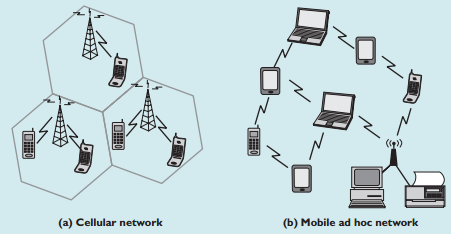
\includegraphics[width=0.8\textwidth]{adhoc.png}
     \caption [Cellular network vs. MANET]{\textbf{Cellular network vs. MANET}. This figure illustrates the difference between a regular cellular network and a mobile ad hoc network \cite{adhoc2}.}
\label{fig:adhoc}
\end{figure}

Mobile ad hoc networks (MANETs) are networks that do not rely on an underlying and fixed infrastructure (access points and routers), in other words "infrastructure-less". MANETs acts in a shared wireless media \cite{adhoc}. The structure of these networks change dynamically. Key factors describing MANETs is self-configuration, self-organization, self-discovery, and self-healing \cite{wmn}. The members of the network are mobile and free to join, or leave, the network at any time \cite{adhoc2}. MANETs are based on multi-hop forwarding. Each node acts not only as a host, but also as a router. The nodes themselves establish and maintain routes, and forward packets to other nodes if necessary. This enables communication between nodes that are originally not within each other's range \cite{adhoc2}. MANETs are suited for use in situations where there are no fixed underlying infrastructure. A MANET can operate as a stand-alone solution, but can also be attached to the Internet. 

\begin{figure}[b]
  \centering
    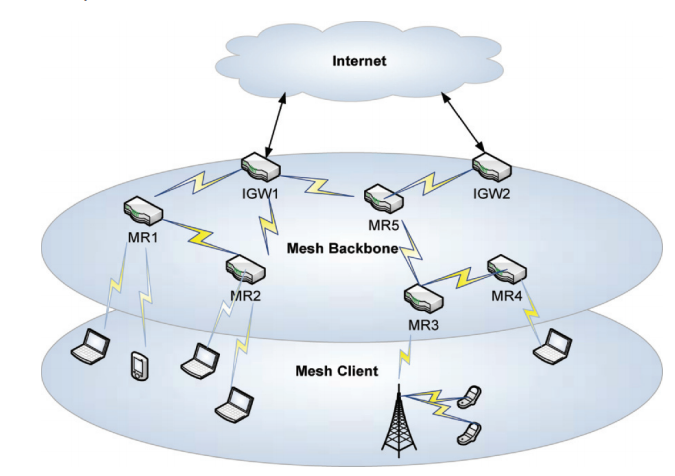
\includegraphics[width=0.8\textwidth]{wmn.png}
     \caption [Example of a Wireless Mesh Network]{\textbf{Example of a Wireless Mesh Network}. This figure illustrates the architecture of a typical WMN \cite{wmn}.}
\label{fig:wmn}
\end{figure}

\subsection{Wireless Mesh Networks}
\label{subsec:mesh}
A wireless mesh network (WMN) is a type of MANET \cite{wmn}. The objective of a WMN is to serve a larger number of users with high bandwidth access. As mentioned before, MANETs are "infrastructure-less" and they have self-configuration, self-organizing, self-healing and self-discovering features. WMNs share all these characteristics, except from the infrastructure part. WMNs are often a collection of routers called mesh routers (MRs). These MRs are usually stationary. The MRs can be employed for different use. One MR could for example be connected via cable to Internet, and then become an Internet gateway. Then this MR can provide Internet connectivity to the other MRs in the mesh network. A wireless mesh network consists of two parts; the backbone of the mesh (the MRs) and the clients of the mesh \cite{wmn}. An example of a WMN architecture is shown in \fref{fig:wmn}. 


\subsection{Routing Protocols}
Ad hoc networks and mesh networks creates several challenges when it comes to routing protocols. The routing protocols must be able to adapt quickly due to the topology changes. \fref{fig:adhocprotocols} shows the different groups of the ad hoc protocols that exist. It is important that a routing protocol do not cause excessive overhead (extensive use of computer resources). Under the category flat routing, there are two types of routing protocols; proactive and reactive. \textit{Proactive routing protocols} (e.g. OLSR) are table driven \citep{proactivereactive}. Every network node has a routing table for forwarding of data. To obtain stability, each node broadcasts and modifies the routing table periodically. Proactive routing protocols are suitable when there are few nodes in the network. The routing table is periodically updated, hence the overhead exceeds the desired value when there are a high number of nodes in the network. In contrary to the proactive routing protocols, \textit{reactive routing protocols} (e.g. AODV) are on demand. Since they are on demand, the overhead is significantly lower. These protocols utilize flooding. The network is flooded with the route request (RREQ) in order to set up the route. The reactive routing protocols do not have a up-to-date routing table like proactive routing protocols \cite{proactivereactive}. Routes are only set up to nodes they communicate with, and these routes are only kept alive while they are needed  \cite{adhoc2}. As shown in \fref{fig:adhocprotocols}, there are several different protocols under proactive and reactive. 


\begin{figure}[t]
  \centering
    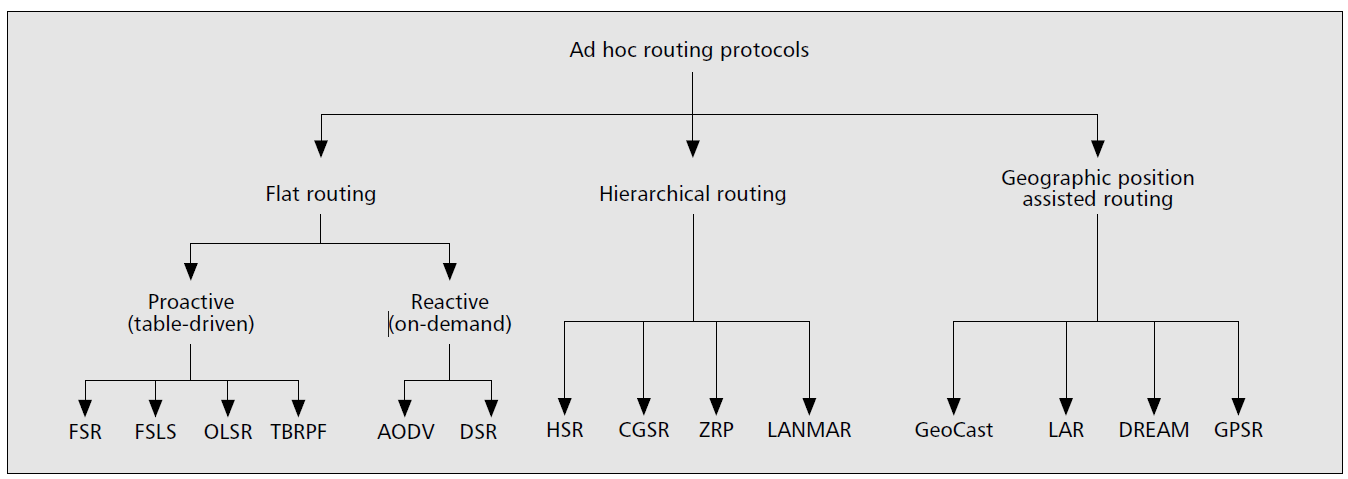
\includegraphics[width=1\textwidth]{adhocprotocols.png}
     \caption[Ad Hoc routing protocols]{\textbf{Different groups of ad hoc routing protocols \cite{adhoc}.}}
\label{fig:adhocprotocols}
\end{figure}


\subsection{B.A.T.M.A.N}
\label{subsec:batman}
Better Approach To Mobile Adhoc Networking (B.A.T.M.A.N) is the routing protocol utilized in the networks formed by the Mesh Potatoes. B.A.T.M.A.N is a proactive routing protocol for wireless ad hoc networks. This includes MANETs \cite{batman}. This protocol was developed as an alternative to OLSR (Optimized Link State Routing) \cite{batman2}. Like mentioned before, routing protocols must be able to adapt quickly to topology changes. B.A.T.M.A.N was made to be a more efficient routing protocol in this area, since it employs a new method for discovering routes. The nodes in the network broadcasts a OGM periodically, like shown in \fref{fig:batman}. A OGM is a Originator Message which contains: 

\begin{itemize}
\item The address of the node
\item Sequence number
\item TTL (Time to live)
\end{itemize}

The address and the sequence number enables identification of a packet and duplicate detection. 

\begin{figure}[b]
  \centering
    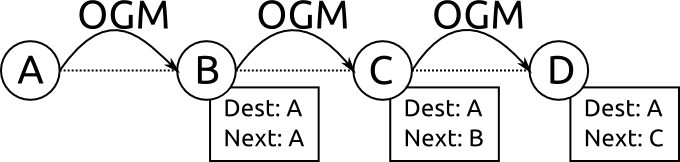
\includegraphics[width=0.8\textwidth]{batman.png}
     \caption[Originator Message in B.A.T.M.A.N]{\textbf{Originator Message used in B.A.T.M.A.N \cite{batman2}.}}
\label{fig:batman} 
\end{figure}


Information about the nodes that are accessible via single-hop or multi-hop are maintained and updated \cite{batman}. Every node updates its routing table each time it receives an OGM. The routing table includes information about \cite{batman2}:

\begin{itemize}
  \item \textbf{Originator Address:} This is the source address of the node that sent the OGM.
  \item \textbf{Current Sequence Number:} The sequence number of the last OGM. This is used to discover if there are any duplicates or any information that is outdated.
  \item \textbf{Sliding Window:} A list of sequence numbers that is stored for each originator and each previous hop, i.e. for the neighbour node that forwarded or originated the OGM, as shown in \fref{fig:batman}. This is used to decide which next hop is best for each destination. 
\end{itemize}

When a node receives an OGM it will decrease the TTL, and then forward it to the neighbour nodes. The same OGM can arrive to a node, but from different paths. In this case, only the first copy is preserved. 

%\subsubsection{RO.B.IN}
%RO.B.IN (Routing Batman Inside) uses the B.A.T.M.A.N routing algorithm. It is a project based on open source, and is intended for wireless mesh networks. It runs on Atheros AP51 routers running OpenWrt. RO.B.IN has the ability to spread wired internet (e.g. DSL) throughout a specific area, for example a village or a school \cite{robin}. 

\subsubsection{Simple Unified Dashboard for mesh networks}
Simple Unified Dashboard (SPUD) for mesh networks is a tool for visualization made for B.A.T.M.A.N mesh networks, and for the users of the networks \cite{spud}. The Simple Unified Dashboard is, like the name indicates, a dashboard based on PHP which is designed to be simple. It communicates with the B.A.T.M.A.N visualization server. The dashboard makes it possible to monitor the link status of the networks, by displaying real time wireless link status. Other features are client management and customization. The software is written in CakePHP and for visualization SPUD uses Google Maps API 1.3 \cite{spud}.

\section{Up-Links}
Our main focus when deploying the emergency box, is to provide Internet to the mesh network. This because it is crucial to have the possibility to communicate with the local community and the outside world during an emergency situation. In 2011, UN declared Internet access a human right \cite{HR}. This says something about the extent of the Internet, and the importance of connectivity. In order to provide Internet to the mesh network formed by the emergency boxes, at least on the Mesh Potatoes must be connected to an access network via an uplink. An uplink connects a device or a LAN to a larger network \cite{uplink}. Which type of access network that is available depends of the location. Some places there might exist a stable landline, other places not. Then an option could be to use satellite or cellular networks. It is therefore important that the emergency box has high adaptability in order to fit different scenarios. The availability of the different uplinks is not the only thing that vary. The up-link speed and the price also varies from place to place, and between the types of uplinks. In the following sections, we will look at some of the uplinks available, and how Internet access can be provided to the mesh network.  

\subsection{Internet via Telephone-line}
The most common way of getting Internet access is via a landline. The telephone lines are most often used for this, since they can be converted to broadband. In this way it can be used for phone calls and Internet simultaneously \cite{internet}. The line is usually in the form of twisted pairs (copper lines). These lines support broadband up to 10 Mbps, and are often in form of ADSL, or other digital subscriber line of type x (xDSL) technologies \citep{audestad}. Internet via telephone lines can be provided as a stand-alone solution, or it can be provided together with television or/and phone service. The latter option is usually cheaper. Internet through landlines have a high reliability \cite{cablevssatellite} in comparison to satellite and cellular network. We will now shorty describe some technologies for getting Internet access via a telephone line; dial-up Internet connection, ISDN, and DSL. Although dial-up Internet connection is practically extinct in developed countries, we will include it here due to the different application scenarios for the emergency box. 

\subsubsection{Dial-up Internet connection}
Dial-up is an analogue technology that utilizes the telephone line. A telephone wall jack is used as a fixed point of connection, and the computer is connected to a voiceband modem. With this technology, the data is transmitted over the same frequencies used for phone calls. Hence, if you only have one telephone line, you cannot take a phone call and use Internet at the same time \cite{differentuplinks}. The absolute maximum speed is 56 kbps. Along with the digital era, better internet technologies were introduced; ISDN and DSL. 

\subsubsection{ISDN}
Integrated Services Digital Network (ISDN) is a fixed internet connection, which also utilizes the telephone lines. When using ISDN, as with dial-up, a telephone wall jack is used as a fixed point of connection. But ISDN utilizes a ISDN terminal adapter instead of voiceband modem. This ISDN terminal adapter sends out digital signals. The data speed varies between 64 kbps - 129 kbps. The speed of the data is symmetric, which means upstream and downstream data rates are the same. In contrary to dial-up, ISDN allows voice calls and transmission of data simultaneously. ISDN is faster than dial-up, but the speed is nothing compared to the speed obtained using DSL \cite{differentuplinks}. 

\subsubsection{DSL}
Digital subscriber line (DSL) is, like the name indicates, a digital high-speed technology for Internet access that allows simultaneous voice and data transfer. Like dial-up and ISDN, DSL also run over the telephone lines. With DSL the data is not converted between analogue and digital signals. Despite this, the signals are modulated in order to be transferred on non-voice frequencies. DSL is an always-on technology, and in this way differ from the previous technologies mentioned. Only a small part of the telephone line is used for voice signals. The DSL technology allows utilization of a unused frequency spectrum of a telephone line, hence making it possible to transmit data faster. When the voice and data signals arrive at the telephone company's local switching station, they are separated and routed differently; voice to regular telephone system and data to the ISP, and then the Internet. A connection must be within approximately 5 kilometres of a station in order for DSL to work. The speed depends on many factors. Data can be transported up to 6 Mbps (distance of approximately 2 kilometres). Relevant factors that have an impact on the speed is distance to the switching station, and the quality of the telephone line. Like mentioned earlier, there are different types of DSLs. The most common is ADSL, where the A stands for asymmetric; the downstream speed is faster than the upstream speed \cite{differentuplinks}.



\subsection{Cellular Network Technologies}

\begin{figure}[b]
  \centering
      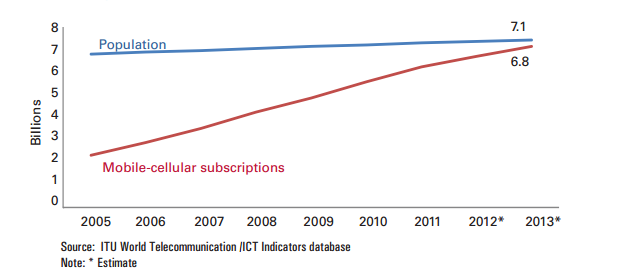
\includegraphics[width=1\textwidth]{mobilesubscriptions.png}
  \caption [Number of mobile-cellular subscriptions]{\textbf{Number of mobile-cellular subscriptions} The figure shows that the growth of mobile-cellular subscriptions have increased drastically during the last decade, and show that there are almost as many as there are people in the world \cite{itu2013}.}
  \label{fig:subscribers}
\end{figure}

%ITU2011-artikkel
It is getting more and more common to use cellular technologies for broadband. Around 2011 the number of mobile-broadband subscriptions grew to twice as many as the number of fixed-broadband subscriptions. In developed countries it is common to have a fixed-broadband connection, and use a mobile-broadband network in addition to the fixed. In developing countries on the other hand, it is not a given that there is access to a fixed-broadband connection. Then mobile-broadband can be the only method of access available. In 2011, 90 \% of the world's population had 2G coverage, and 45 \% had 3G coverage \cite{itu2011}. By 2013, the number of mobile-cellular subscriptions had reached a high level, and were approaching the number of people in the world, like shown in \fref{fig:subscribers}. From 2011 to 2013, the number of mobile-broadband  subscriptions more than doubled in developing countries \cite{itu2013}. 

Through mobile network technologies, high-speed Internet access can be provided via portable devices. In order to get mobile broadband, there must be a cellular network (GSM, CDMA) service available. The key technologies when talking about mobile broadband is 3G and 4G (respectively third and fourth generation wireless networks) \cite{mobilebroadband}. With 3G the average speed is 0.5 to 1.5 Mbps, and with 4G the average speed is 2 to 12 Mbps. These vary, due to different versions of each technology, underlying service etc. Like with everything else, the actual and realistic speed differ from the peak speed \cite{3gvs4g}. 


\subsection{Satellite}
%ulovlig i feks india, hva skjer da? http://en.wikipedia.org/wiki/Satellite_phone
Internet from satellites are offered by a satellite Internet provider \cite{cablevssatellite}. The satellite are orbiting the Earth, and get signals from a land based Internet connection. To get Internet broadband via satellite you need a satellite dish. The main advantage of using satellite is that it provides an universally available Internet access \cite{broadband}. Since it is universally available, it is fitted for use in rural regions where there exists no landlines or other options for connecting to the Internet. There also exists disadvantages with using satellite-Internet. Since it is a shared medium, privacy concerns arise, and the speed are dependent of simultaneous use. Also the connection can be affected by bad weather, unlike for a wired connection, hence it is not as reliable as cable. 


\subsection{Summary Up-Links}

\begin{center}
\begin{table}[!h]
\caption{\label{tab:uplinks}Advantages and disadvantages - Up-links \cite{comparisonuplinks}.}
    \begin{tabular}{ | l | p{4cm} | p{5cm} |}
    \hline
    \textbf{Up-links} & \textbf{Advantages} & \textbf{Disadvantages} \\ 
    \hline
    Landline/xDSL & High reliability, cost effective, good speed. & Low availability in rural areas. \\ 
    \hline
     Cellular networks & High availability, fitted for "on the move"-use. & Expensive, slower than xDSL.\\
    \hline
    Satellite & High availability.  & Unreliable, expensive, slower than landline.\\ 
    \hline
    \end{tabular}
   \end{table}
\end{center}


\section{Future Internet Access Methods}
Different methods of distributing Internet is always under development. The previous up-links described is well established, but in many parts of the world not fully developed or not affordable to the average person. The large technology companies, like Google, are experimenting with different ways of distributing Internet. 

\subsection{Google's Internet Balloons}
The majority of the world today is not connected to the Internet. Two thirds of the worlds population does not have access. Project Loon, a Google project, is a network of high altitude balloons travelling in the stratosphere, and through this network be able to give Internet to the Entire world. Cost effective, reliable and inexpensive internet connection to everybody. The project started in June 2013 as a experiment in New Zealand \cite{loon}. 

\begin{figure}
        \centering
        \begin{subfigure}[t]{0.43\textwidth}
                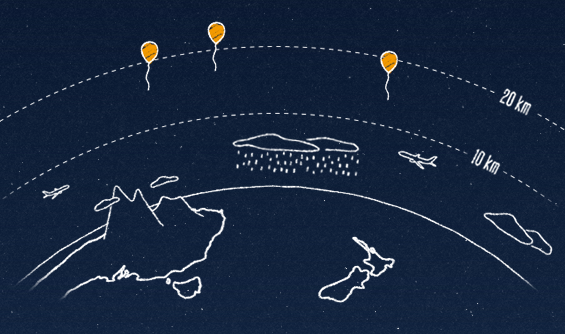
\includegraphics[width=\textwidth]{loon2.PNG}
                \caption[The Balloons are situated in the stratosphere]{\textbf{The Balloons are situated in the stratosphere.}} 
                \label{fig:loonStratosphere}
        \end{subfigure}%
        ~ %add desired spacing between images, e. g. ~, \quad, \qquad etc.
          %(or a blank line to force the subfigure onto a new line)
        \begin{subfigure}[t]{0.415\textwidth}
                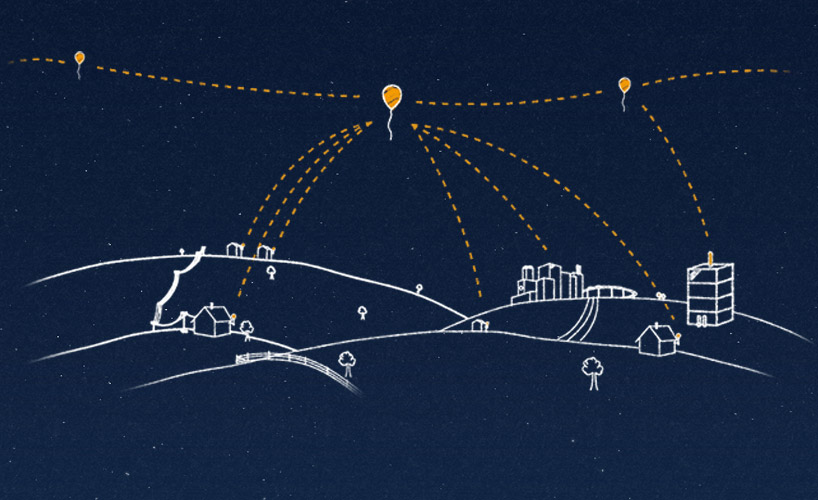
\includegraphics[width=\textwidth]{loon1.jpg}
               \caption[Connecting to the Internet]							{\textbf{Connecting to the Internet}} 
                \label{fig:loonConnect}
        \end{subfigure}
        ~ %add desired spacing between images, e. g. ~, \quad, \qquad etc.
          %(or a blank line to force the subfigure onto a new line)
        \caption{Project Loon: Balloon-powered internet for everyone.}\label{fig:loon}
\end{figure}

The balloons are 15 meter in diameter. They travel about 20 km up in the air, in the stratosphere, twice as high as airplanes and weather, this is shown in \fref{fig:loonStratosphere}. At this altitude there are many layers of wind, each varies in direction and speed. By regulating which wind the balloons are flying in it is possible to control their position, and steer them in the desired direction. \fref{fig:loonConnect} show that  people can connect to the Internet shared by the balloons by having a special antenna attached to their house. From this antenna the signal bounces to one balloon which again bounces through the other balloons and down to the Local Internet Provider on earth. This creates a network in the sky. 

In order to control the altitude of the balloon, it is a specially designed control system. The system is managed remotely from the ground. By either pumping air in, or letting air out of the balloon, one can decide in what layer of air the balloon should be in. Letting air in and out is not the only way to decide whether the balloon should go up or down, but it is the only way to do so in huge scale. A GPS is attached to each balloon in order to keep track of precise positions and see how the winds are changing. There are enormous amounts of data collected, and some of this information is given to meteorologists. The balloons are flying at the same speed as the wind.  

The balloons contains specially designed antennas and radio systems. This in order to receive signals from Project Loon only, and to achieve high bandwidth over long distances. Satellites stay at the same place and at the same altitude. This means that the satellite dish can be mounted in the right direction. This is not the case with the balloons, they are in constant movement and they also vary in attitude. A fixed pointing dish would therefore not work. The antenna needs more sensitivity to an angle than it does straight up, which results in a uniform signal strength. 

Since the balloons are in constant movement, it is important to make sure that there always is a balloon available and one ready to move in when one move out so that the connectivity always are available. If not this project would not be of much use. Every balloon contains information about all the other balloons in order to spread out nicely. Think of it as a flock of birds, they always look at the one next to them and space out perfectly.

The balloons are solely run on solar power. The balloon works as a communication tower in the sky. The solar panels catches the sunlight that is available during the day, as well as charging up the lithium-ion battery to last the night. In the stratosphere it is -70 degrees Celsius, these extreme cold conditions are not ideal fro the lithium battery. In order to make sure that the battery does not loose its effective battery capacity it is important that the battery is kept warm. The battery pack is insulated to reflect the heat that comes of the electronics to stay warm. This is still under development. 

When it comes to lifetime, the goal is that the balloons stay alive for 100 days, or 3 laps around the globe. It is important to make sure that the balloon is leak free. The material is under a lot of stress, air is constantly being pumped in and out to control the position. As well as the extreme cold and warm temperatures. 

Both on the way up and down the air traffic control in the specific country have to be contacted since the balloons go through airspace. Project loon requested permission to land on Norwegian soil according to Teknisk Ukeblad, a Norwegian science magazine. This permission was approved \cite{loonTU}.

The area of usage is enormous. Situations where the Internet infrastructure has not been built out, either because it is too expensive or just not possible. Emergency situations, natural disaster and other situations where the cellphone-towers are down. Project Loon is still a project in development with extensive testing taking place. The project are taking into use what everybody have in common, namely the sky, to reach out to all the areas where access has not been possible. It is expensive to have enough balloons in the sky in order to have good enough coverage. Also the speed is not really high. And even though a specialized antenna is required to get access, this is breakthrough in order to get the whole world connected \cite{loonYouTube, loonNorsk}.

Although this solution is not an option for distributing Internet as of today, it could be a good option in the near future. The solution is affordable and well compatible with our emergency box solution.

Iridium satellite consultation is a large group of satellites providing data and and voice services to specialized satellite phones. The consultation exists of 66 active satellites in orbit. Iridium are considered to be low-orbit satellites and are situated at a hight of 781 km. The Iridium network is unique in the fact that it covers the whole earth, including oceans, airways and poles. The low orbit satellite differs from the balloons in the way that the satellites travel almost 40 times higher above earth and that they stay in a fixed position over the earth \cite{iridium}. To be able to utilize the satellite one would need a specialized satellite phone or a satellite dish in order to receive signal. With the balloons there are only need for an antenna to receive the signal. But then again the balloons does not offer a voice service. The balloons are intended as a cheaper, easier and simpler solution to the satellites.                                         

\section{Apple's Mesh Network}
In March 2014 a new iOS app was released, FireChat. FireChat utilizes Apple's Multipeer Connectivity Framework introduced in iOS7 \cite{appleMesh}. This app enables the possibility to chat with people "off-the-grid" \cite{fireChat}. Applications that communicates through this framework creates a mesh network similar to the one created by the Mesh Potatoes. 

The Multipeer Connectivity framework provides support for discovering services provided by nearby iOS devices using peer-to-peer Wi-Fi, infrastructure Wi-Fi networks and bluetooth to communicate with those services. This communication could either be message-based data, streaming data and resources such as files \cite{multipeer}. These technologies have a short range, but this range can be greatly extended by a chain of users that creates a mesh network, see section \ref{subsec:mesh} for more information about mesh networks. AirDrop is a product that have been on the market for a while and also utilizes mesh networks. The main difference is that FireChat is fully decentralized and peer-to-peer. When there are multiple users in one area FireChat relay messages in the same way as Internet, from node to node, just in this case it is from phone to phone.  This, not only, enables two users to chat with each other without Internet connection, but also far beyond Wi-Fi and Bluetooth range from each other, using the chain of users (phones). For example if Bob is connected to Alice, and Alice is connected to Carol, Bob and Carol can send messages to each other. This chain can be indefinitely long. As long as no one device goes out of Wi-Fi range, all the devices can communicate with each other. 

This new framework will mainstream wireless mesh networking. This could open for a future way of spreading Internet access. This could for example be a hotel basement, cave or rural areas where there are no cellphone towers, or disaster situations where Wi-Fi or mobile broadband  is no longer available. There are many benefits with the use of mesh networks. Mesh networks does not require a centralized infrastructure, there are no need for all the devices to be connected to Internet (as a router). Another benefit is that the mesh network is really easy to set up - everybody just uses the app FireChat (or similar applications like AirDrop), the network is created and everybody is connected. Simple as that! 

The possibilities for this feature are enormous. Both in the creation of applications but also the area of usage. In a lot of countries Internet and mobile broadband connection is extremely expensive, people might afford a used cellphone but not the cost to connect. With this new feature, Internet connectivity can be spread through the mesh network needing only one node (phone) to have internet access. This way of spreading connectivity can open the possibility for people in rural, poorer areas like slums and small villages to stay connected. But not only the poor and rural areas can benefit from this new mesh-networking feature. Young people that does not have a phone can use an iPad or similar to talk to their friends. Or teens with restricted cell contracts can still connect with their friends, just with the help of the neighbours kids phone. Since FireChat enables communication without the use of internet it can be a useful tool to communicate privately and also to send sensitive data.
 
It is not only Apple that is seizing the enormous potential in main-streaming mesh networking. Google has also expressed that they are working on a home mesh network \cite{googleMesh}. FireChat and AirDrop is just the beginning. We believe more extensive and mind blowing applications are to come. 


